\chapter{Test Journal: Inner Controller} \label{app:Inner}

\textbf{Date: 26/05/2017}

\subsection*{Purpose}
Check the performance of the inner controller, when tracking references in $\dot{x}_\mathrm{b}$ and $\psi$.

\subsection*{Equipment}
\begin{itemize}
    \item Vessel with all its components. 
    \item External laptop.
\end{itemize}

\subsection*{Procedure}
\begin{enumerate}
    \item Turn on all equipment.
    \item Remotely log into the vessel, when both, laptop and vessel's computer, are in the same network.
    \item Run the following nodes
    \begin{itemize}
        \item \lstinline[style=cinline]{/lli_node}
        \item \lstinline[style=cinline]{/sensor_node}
        \item \lstinline[style=cinline]{/gps1_node} (adapted to work with a previous implementation of the Kalman filter)
        \item \lstinline[style=cinline]{/KF_attitude_node}
        \item \lstinline[style=cinline]{/kalmanfilter_node} (from a previous implementation)
    \end{itemize}
    \item Record the following topics
    \begin{itemize}
        \item \lstinline[style=cinline]{/imu}   
        \item \lstinline[style=cinline]{/gps1} (from a previous implementation)
        \item \lstinline[style=cinline]{/kf_attitude}
        \item \lstinline[style=cinline]{/KF_States} (from a previous implementation)  
        \item \lstinline[style=cinline]{/lli_input}  
    \end{itemize}
    \item Run the \lstinline[style=cinline]{/controller_node} with a reference in $\psi$ and $\dot{x}_\mathrm{b}$.
    \item Stop the recording after some time has passed.
    \item Turn off the equipment.
    \item Process the data.
\end{enumerate}

\subsection*{Results}
The results of the test can be seen in \autoref{fig:inner_yaw_app} and \ref{fig:inner_xbdot_app}.
\begin{figure}[H]
    \captionbox 
    {   
        Response in $\psi$ with a reference of -1 rad.
        \label{fig:inner_yaw_app}
    }                                                                 
    {                                                                  
        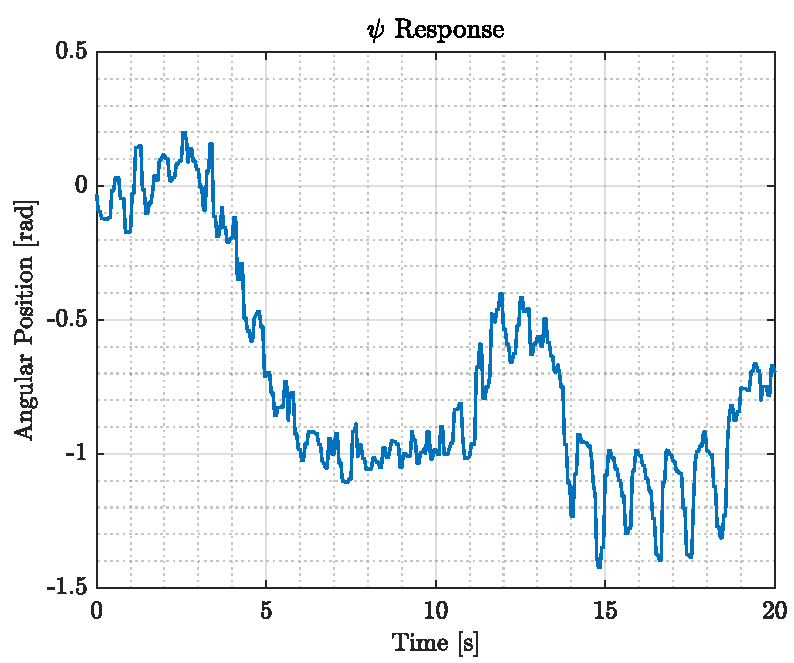
\includegraphics[width=.45\textwidth]{figures/inner_yaw}         
    }                                                                    
    \hspace{5pt}                                                          
    \captionbox  
    {      
        Reponse in $\dot{x}_\mathrm{b}$ with a reference of 1 m$\cdot$s$^{-1}$.
        \label{fig:inner_xbdot_app}
    }                                                                          
    {
        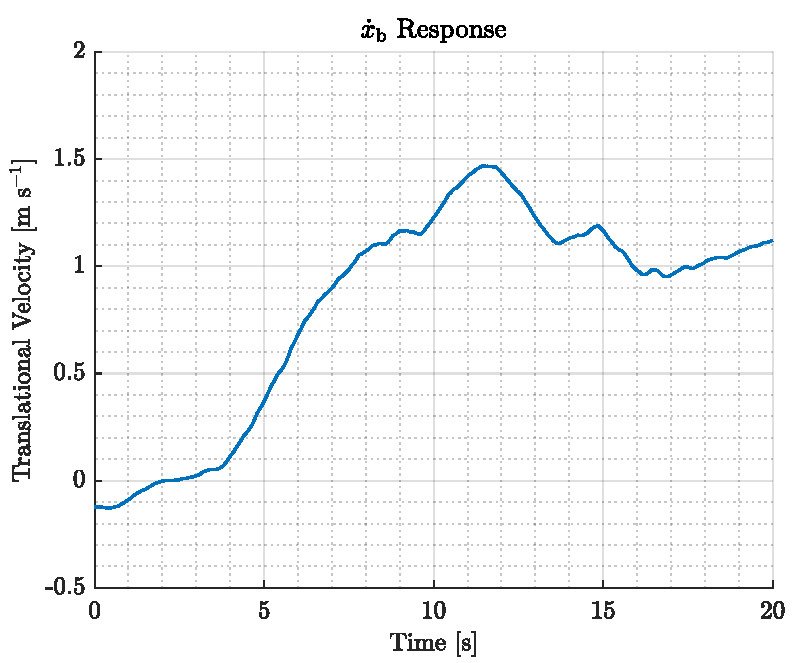
\includegraphics[width=.45\textwidth]{figures/inner_xbdot}
    }
\end{figure}

